\documentclass[leqno, 12pt]{article}
\usepackage{tikz}
\usepackage{amsmath}
\usepackage{ulem}
\usetikzlibrary{angles,quotes,intersections,arrows.meta,calc}
\usepackage[a4paper, portrait, margin=1cm]{geometry}
\usepackage{multicol}
\usepackage{fancyhdr}

\def \HeadingAnswers {\section*{\Large Name: \underline{\hspace{8cm}} \hfill Date: \underline{\hspace{3cm}}} \vspace{-3mm}
{Parallel lines : Answers} \vspace{1pt}\hrule}

% raise footer with page number; no header
\fancypagestyle{myfancypagestyle}{
  \fancyhf{}% clear all header and footer fields
  \renewcommand{\headrulewidth}{0pt} % no rule under header
  \fancyfoot[C] {\thepage} \setlength{\footskip}{14.5pt} % raise page number 6pt
}
\pagestyle{myfancypagestyle}  % apply myfancypagestyle

\newcounter{minipagecount}

\begin{document}
\HeadingAnswers
\begin{multicols}{2}


\begin{equation}
  \text{e} = \text{147}^\circ
  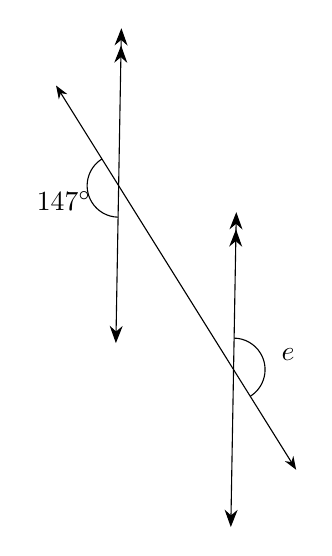
\begin{tikzpicture}[scale=1.0, baseline=(current bounding box.north)]
    \begin{scope}[rotate=302]
      % Draw the first line
      \draw[<->>, >={Stealth[scale=1.3]}, name path=P1] (0, 0) -- (-3.3546822717816958, 2.1785561400601092);
      % Draw the second line with the calculated offsets
      \draw[<->>, >={Stealth[scale=1.3]}, name path=P2] (2.754117688164994, 0) -- (-0.600564583616702, 2.1785561400601092);
      % Draw the transversal through the middle of the parallel lines
      \draw[<->, >=Stealth, name path=P3] (-3.177341135890848, 1.0892780700300546) -- (2.576776552274146, 1.0892780700300546);
      \path [name intersections={of=P1 and P3,by=A}];
      \path [name intersections={of=P2 and P3,by=B}];
      % Draw the angle
      \coordinate (p1s) at (0, 0);
      \coordinate (p1e) at (-3.3546822717816958, 2.1785561400601092);
      \coordinate (p2s) at (2.754117688164994, 0);
      \coordinate (p2e) at (-0.600564583616702, 2.1785561400601092);
      \coordinate (ts) at (-3.177341135890848, 1.0892780700300546);
      \coordinate (te) at (2.576776552274146, 1.0892780700300546);
      \draw pic["$e$", draw=black, -, angle eccentricity=1.8, angle radius=0.4cm] {angle=te--B--p2e};
\draw pic["$147^\circ$", draw=black, -, angle eccentricity=1.8, angle radius=0.4cm] {angle=ts--A--p1s};

    \end{scope}
  \end{tikzpicture}
\end{equation}\vspace{1cm}
\begin{equation}
  \text{f} = \text{150}^\circ
  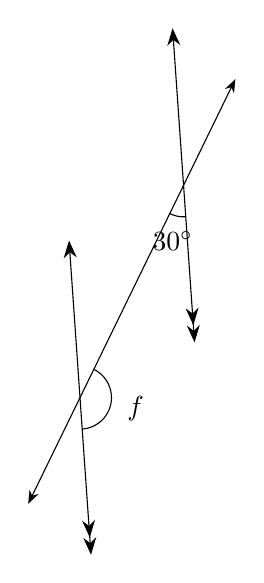
\begin{tikzpicture}[scale=1.0, baseline=(current bounding box.north)]
    \begin{scope}[rotate=244]
      % Draw the first line
      \draw[<->>, >={Stealth[scale=1.3]}, name path=P1] (0, 0) -- (3.464101615137755, 1.9999999999999998);
      % Draw the second line with the calculated offsets
      \draw[<->>, >={Stealth[scale=1.3]}, name path=P2] (3.0000000000000004, 0) -- (6.464101615137755, 1.9999999999999998);
      % Draw the transversal through the middle of the parallel lines
      \draw[<->, >=Stealth, name path=P3] (0.23205080756887764, 0.9999999999999999) -- (6.232050807568878, 0.9999999999999999);
      \path [name intersections={of=P1 and P3,by=A}];
      \path [name intersections={of=P2 and P3,by=B}];
      % Draw the angle
      \coordinate (p1s) at (0, 0);
      \coordinate (p1e) at (3.464101615137755, 1.9999999999999998);
      \coordinate (p2s) at (3.0000000000000004, 0);
      \coordinate (p2e) at (6.464101615137755, 1.9999999999999998);
      \coordinate (ts) at (0.23205080756887764, 0.9999999999999999);
      \coordinate (te) at (6.232050807568878, 0.9999999999999999);
      \draw pic["$f$", draw=black, -, angle eccentricity=1.8, angle radius=0.4cm] {angle=p2e--B--ts};
\draw pic["$30^\circ$", draw=black, -, angle eccentricity=1.8, angle radius=0.4cm] {angle=te--A--p1e};

    \end{scope}
  \end{tikzpicture}
\end{equation}\vspace{1cm}
\begin{equation}
  \text{h} = \text{56}^\circ
  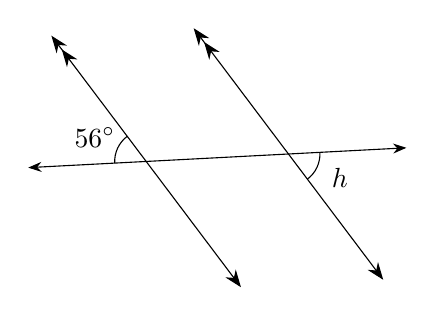
\begin{tikzpicture}[scale=1.0, baseline=(current bounding box.north)]
    \begin{scope}[rotate=3]
      % Draw the first line
      \draw[<->>, >={Stealth[scale=1.3]}, name path=P1] (0, 0) -- (-2.2367716138829867, 3.316150290220167);
      % Draw the second line with the calculated offsets
      \draw[<->>, >={Stealth[scale=1.3]}, name path=P2] (1.809326922755858, 0) -- (-0.4274446911271288, 3.316150290220167);
      % Draw the transversal through the middle of the parallel lines
      \draw[<->, >=Stealth, name path=P3] (-2.618385806941493, 1.6580751451100835) -- (2.190941115814365, 1.6580751451100835);
      \path [name intersections={of=P1 and P3,by=A}];
      \path [name intersections={of=P2 and P3,by=B}];
      % Draw the angle
      \coordinate (p1s) at (0, 0);
      \coordinate (p1e) at (-2.2367716138829867, 3.316150290220167);
      \coordinate (p2s) at (1.809326922755858, 0);
      \coordinate (p2e) at (-0.4274446911271288, 3.316150290220167);
      \coordinate (ts) at (-2.618385806941493, 1.6580751451100835);
      \coordinate (te) at (2.190941115814365, 1.6580751451100835);
      \draw pic["$h$", draw=black, -, angle eccentricity=1.8, angle radius=0.4cm] {angle=p2s--B--te};
\draw pic["$56^\circ$", draw=black, -, angle eccentricity=1.8, angle radius=0.4cm] {angle=p1e--A--ts};

    \end{scope}
  \end{tikzpicture}
\end{equation}\vspace{1cm}
\begin{equation}
  \text{a} = \text{75}^\circ
  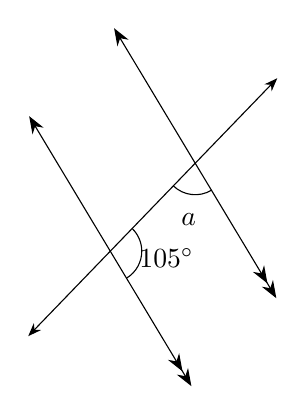
\begin{tikzpicture}[scale=1.0, baseline=(current bounding box.north)]
    \begin{scope}[rotate=226]
      % Draw the first line
      \draw[<->>, >={Stealth[scale=1.3]}, name path=P1] (0, 0) -- (1.035276180410083, 3.8637033051562732);
      % Draw the second line with the calculated offsets
      \draw[<->>, >={Stealth[scale=1.3]}, name path=P2] (1.5529142706151244, 0) -- (2.5881904510252074, 3.8637033051562732);
      % Draw the transversal through the middle of the parallel lines
      \draw[<->, >=Stealth, name path=P3] (-0.9823619097949585, 1.9318516525781366) -- (3.570552360820166, 1.9318516525781366);
      \path [name intersections={of=P1 and P3,by=A}];
      \path [name intersections={of=P2 and P3,by=B}];
      % Draw the angle
      \coordinate (p1s) at (0, 0);
      \coordinate (p1e) at (1.035276180410083, 3.8637033051562732);
      \coordinate (p2s) at (1.5529142706151244, 0);
      \coordinate (p2e) at (2.5881904510252074, 3.8637033051562732);
      \coordinate (ts) at (-0.9823619097949585, 1.9318516525781366);
      \coordinate (te) at (3.570552360820166, 1.9318516525781366);
      \draw pic["$a$", draw=black, -, angle eccentricity=1.8, angle radius=0.4cm] {angle=te--A--p1e};
\draw pic["$105^\circ$", draw=black, -, angle eccentricity=1.8, angle radius=0.4cm] {angle=p2e--B--ts};

    \end{scope}
  \end{tikzpicture}
\end{equation}\vspace{1cm}
\begin{equation}
  \text{g} = \text{104}^\circ
  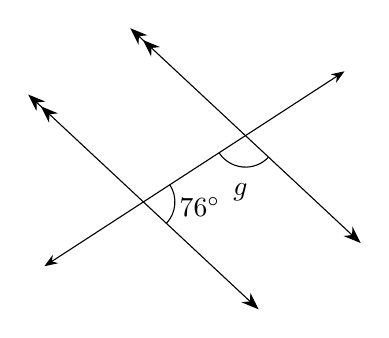
\begin{tikzpicture}[scale=1.0, baseline=(current bounding box.north)]
    \begin{scope}[rotate=33]
      % Draw the first line
      \draw[<->>, >={Stealth[scale=1.3]}, name path=P1] (0, 0) -- (-0.9676875823986711, 3.881182905103986);
      % Draw the second line with the calculated offsets
      \draw[<->>, >={Stealth[scale=1.3]}, name path=P2] (1.545920444024847, 0) -- (0.5782328616261759, 3.881182905103986);
      % Draw the transversal through the middle of the parallel lines
      \draw[<->, >=Stealth, name path=P3] (-1.9838437911993354, 1.940591452551993) -- (2.5620766528255112, 1.940591452551993);
      \path [name intersections={of=P1 and P3,by=A}];
      \path [name intersections={of=P2 and P3,by=B}];
      % Draw the angle
      \coordinate (p1s) at (0, 0);
      \coordinate (p1e) at (-0.9676875823986711, 3.881182905103986);
      \coordinate (p2s) at (1.545920444024847, 0);
      \coordinate (p2e) at (0.5782328616261759, 3.881182905103986);
      \coordinate (ts) at (-1.9838437911993354, 1.940591452551993);
      \coordinate (te) at (2.5620766528255112, 1.940591452551993);
      \draw pic["$g$", draw=black, -, angle eccentricity=1.8, angle radius=0.4cm] {angle=ts--B--p2s};
\draw pic["$76^\circ$", draw=black, -, angle eccentricity=1.8, angle radius=0.4cm] {angle=p1s--A--te};

    \end{scope}
  \end{tikzpicture}
\end{equation}\vspace{1cm}
\begin{equation}
  \text{c} = \text{116}^\circ
  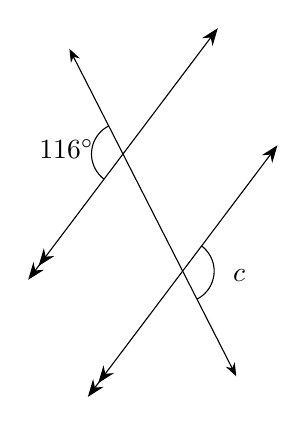
\begin{tikzpicture}[scale=1.0, baseline=(current bounding box.north)]
    \begin{scope}[rotate=117]
      % Draw the first line
      \draw[<->>, >={Stealth[scale=1.3]}, name path=P1] (0, 0) -- (-1.75348458715631, 3.5951761851966677);
      % Draw the second line with the calculated offsets
      \draw[<->>, >={Stealth[scale=1.3]}, name path=P2] (1.6689029107127835, 0) -- (-0.08458167644352654, 3.5951761851966677);
      % Draw the transversal through the middle of the parallel lines
      \draw[<->, >=Stealth, name path=P3] (-2.376742293578155, 1.7975880925983339) -- (2.2921606171346287, 1.7975880925983339);
      \path [name intersections={of=P1 and P3,by=A}];
      \path [name intersections={of=P2 and P3,by=B}];
      % Draw the angle
      \coordinate (p1s) at (0, 0);
      \coordinate (p1e) at (-1.75348458715631, 3.5951761851966677);
      \coordinate (p2s) at (1.6689029107127835, 0);
      \coordinate (p2e) at (-0.08458167644352654, 3.5951761851966677);
      \coordinate (ts) at (-2.376742293578155, 1.7975880925983339);
      \coordinate (te) at (2.2921606171346287, 1.7975880925983339);
      \draw pic["$c$", draw=black, -, angle eccentricity=1.8, angle radius=0.4cm] {angle=ts--A--p1s};
\draw pic["$116^\circ$", draw=black, -, angle eccentricity=1.8, angle radius=0.4cm] {angle=te--B--p2e};

    \end{scope}
  \end{tikzpicture}
\end{equation}\vspace{1cm}
\begin{equation}
  \text{d} = \text{137}^\circ
  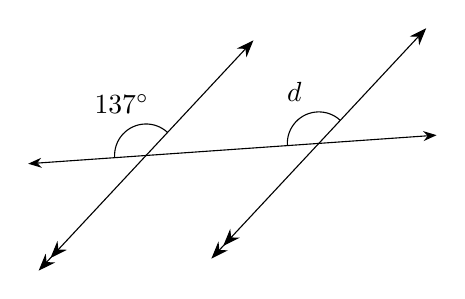
\begin{tikzpicture}[scale=1.0, baseline=(current bounding box.north)]
    \begin{scope}[rotate=184]
      % Draw the first line
      \draw[<->>, >={Stealth[scale=1.3]}, name path=P1] (0, 0) -- (2.925414806476682, 2.727993440249994);
      % Draw the second line with the calculated offsets
      \draw[<->>, >={Stealth[scale=1.3]}, name path=P2] (2.1994187784594375, 0) -- (5.12483358493612, 2.727993440249994);
      % Draw the transversal through the middle of the parallel lines
      \draw[<->, >=Stealth, name path=P3] (-0.037292596761658636, 1.363996720124997) -- (5.162126181697778, 1.363996720124997);
      \path [name intersections={of=P1 and P3,by=A}];
      \path [name intersections={of=P2 and P3,by=B}];
      % Draw the angle
      \coordinate (p1s) at (0, 0);
      \coordinate (p1e) at (2.925414806476682, 2.727993440249994);
      \coordinate (p2s) at (2.1994187784594375, 0);
      \coordinate (p2e) at (5.12483358493612, 2.727993440249994);
      \coordinate (ts) at (-0.037292596761658636, 1.363996720124997);
      \coordinate (te) at (5.162126181697778, 1.363996720124997);
      \draw pic["$d$", draw=black, -, angle eccentricity=1.8, angle radius=0.4cm] {angle=p1s--A--te};
\draw pic["$137^\circ$", draw=black, -, angle eccentricity=1.8, angle radius=0.4cm] {angle=p2s--B--te};

    \end{scope}
  \end{tikzpicture}
\end{equation}\vspace{1cm}
\begin{equation}
  \text{e} = \text{96}^\circ
  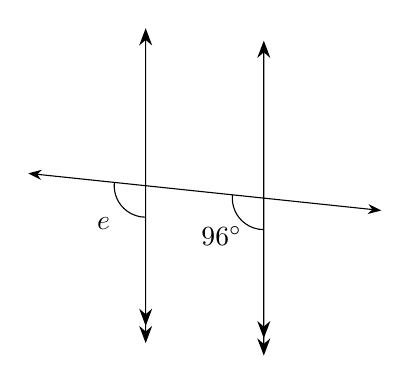
\begin{tikzpicture}[scale=1.0, baseline=(current bounding box.north)]
    \begin{scope}[rotate=174]
      % Draw the first line
      \draw[<->>, >={Stealth[scale=1.3]}, name path=P1] (0, 0) -- (-0.4181138530706142, 3.978087581473093);
      % Draw the second line with the calculated offsets
      \draw[<->>, >={Stealth[scale=1.3]}, name path=P2] (1.5082624193452747, 0) -- (1.0901485662746606, 3.978087581473093);
      % Draw the transversal through the middle of the parallel lines
      \draw[<->, >=Stealth, name path=P3] (-1.7090569265353073, 1.9890437907365466) -- (2.7992054928099677, 1.9890437907365466);
      \path [name intersections={of=P1 and P3,by=A}];
      \path [name intersections={of=P2 and P3,by=B}];
      % Draw the angle
      \coordinate (p1s) at (0, 0);
      \coordinate (p1e) at (-0.4181138530706142, 3.978087581473093);
      \coordinate (p2s) at (1.5082624193452747, 0);
      \coordinate (p2e) at (1.0901485662746606, 3.978087581473093);
      \coordinate (ts) at (-1.7090569265353073, 1.9890437907365466);
      \coordinate (te) at (2.7992054928099677, 1.9890437907365466);
      \draw pic["$e$", draw=black, -, angle eccentricity=1.8, angle radius=0.4cm] {angle=te--B--p2e};
\draw pic["$96^\circ$", draw=black, -, angle eccentricity=1.8, angle radius=0.4cm] {angle=te--A--p1e};

    \end{scope}
  \end{tikzpicture}
\end{equation}\vspace{1cm}
\begin{equation}
  \text{f} = \text{75}^\circ
  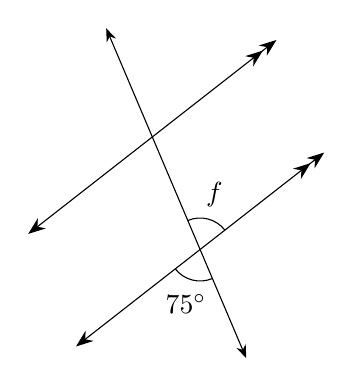
\begin{tikzpicture}[scale=1.0, baseline=(current bounding box.north)]
    \begin{scope}[rotate=293]
      % Draw the first line
      \draw[<->>, >={Stealth[scale=1.3]}, name path=P1] (0, 0) -- (-1.0352761804100834, 3.8637033051562732);
      % Draw the second line with the calculated offsets
      \draw[<->>, >={Stealth[scale=1.3]}, name path=P2] (1.5529142706151244, 0) -- (0.517638090205041, 3.8637033051562732);
      % Draw the transversal through the middle of the parallel lines
      \draw[<->, >=Stealth, name path=P3] (-2.0176380902050415, 1.9318516525781366) -- (2.535276180410083, 1.9318516525781366);
      \path [name intersections={of=P1 and P3,by=A}];
      \path [name intersections={of=P2 and P3,by=B}];
      % Draw the angle
      \coordinate (p1s) at (0, 0);
      \coordinate (p1e) at (-1.0352761804100834, 3.8637033051562732);
      \coordinate (p2s) at (1.5529142706151244, 0);
      \coordinate (p2e) at (0.517638090205041, 3.8637033051562732);
      \coordinate (ts) at (-2.0176380902050415, 1.9318516525781366);
      \coordinate (te) at (2.535276180410083, 1.9318516525781366);
      \draw pic["$f$", draw=black, -, angle eccentricity=1.8, angle radius=0.4cm] {angle=p2e--B--ts};
\draw pic["$75^\circ$", draw=black, -, angle eccentricity=1.8, angle radius=0.4cm] {angle=p2s--B--te};

    \end{scope}
  \end{tikzpicture}
\end{equation}\vspace{1cm}
\begin{equation}
  \text{f} = \text{90}^\circ
  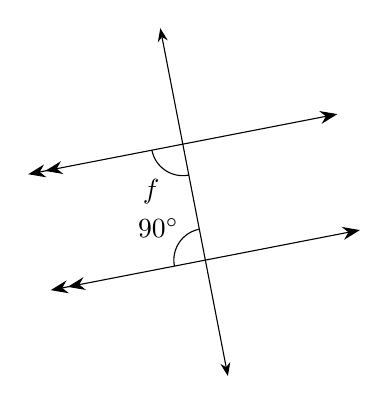
\begin{tikzpicture}[scale=1.0, baseline=(current bounding box.north)]
    \begin{scope}[rotate=101]
      % Draw the first line
      \draw[<->>, >={Stealth[scale=1.3]}, name path=P1] (0, 0) -- (2.4492935982947064e-16, 4.0);
      % Draw the second line with the calculated offsets
      \draw[<->>, >={Stealth[scale=1.3]}, name path=P2] (1.5, 0) -- (1.5000000000000002, 4.0);
      % Draw the transversal through the middle of the parallel lines
      \draw[<->, >=Stealth, name path=P3] (-1.5, 2.0) -- (3.0, 2.0);
      \path [name intersections={of=P1 and P3,by=A}];
      \path [name intersections={of=P2 and P3,by=B}];
      % Draw the angle
      \coordinate (p1s) at (0, 0);
      \coordinate (p1e) at (2.4492935982947064e-16, 4.0);
      \coordinate (p2s) at (1.5, 0);
      \coordinate (p2e) at (1.5000000000000002, 4.0);
      \coordinate (ts) at (-1.5, 2.0);
      \coordinate (te) at (3.0, 2.0);
      \draw pic["$f$", draw=black, -, angle eccentricity=1.8, angle radius=0.4cm] {angle=p2e--B--ts};
\draw pic["$90^\circ$", draw=black, -, angle eccentricity=1.8, angle radius=0.4cm] {angle=te--A--p1e};

    \end{scope}
  \end{tikzpicture}
\end{equation}\vspace{1cm}
\begin{equation}
  \text{a} = \text{115}^\circ
  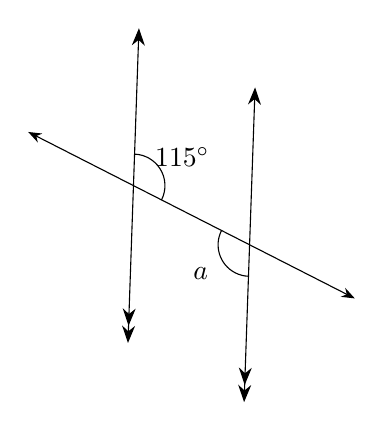
\begin{tikzpicture}[scale=1.0, baseline=(current bounding box.north)]
    \begin{scope}[rotate=153]
      % Draw the first line
      \draw[<->>, >={Stealth[scale=1.3]}, name path=P1] (0, 0) -- (-1.6904730469627973, 3.6252311481466);
      % Draw the second line with the calculated offsets
      \draw[<->>, >={Stealth[scale=1.3]}, name path=P2] (1.6550668784437375, 0) -- (-0.035406168519059866, 3.6252311481466);
      % Draw the transversal through the middle of the parallel lines
      \draw[<->, >=Stealth, name path=P3] (-2.345236523481399, 1.8126155740733) -- (2.309830354962339, 1.8126155740733);
      \path [name intersections={of=P1 and P3,by=A}];
      \path [name intersections={of=P2 and P3,by=B}];
      % Draw the angle
      \coordinate (p1s) at (0, 0);
      \coordinate (p1e) at (-1.6904730469627973, 3.6252311481466);
      \coordinate (p2s) at (1.6550668784437375, 0);
      \coordinate (p2e) at (-0.035406168519059866, 3.6252311481466);
      \coordinate (ts) at (-2.345236523481399, 1.8126155740733);
      \coordinate (te) at (2.309830354962339, 1.8126155740733);
      \draw pic["$a$", draw=black, -, angle eccentricity=1.8, angle radius=0.4cm] {angle=te--A--p1e};
\draw pic["$115^\circ$", draw=black, -, angle eccentricity=1.8, angle radius=0.4cm] {angle=ts--B--p2s};

    \end{scope}
  \end{tikzpicture}
\end{equation}\vspace{1cm}
\begin{equation}
  \text{e} = \text{87}^\circ
  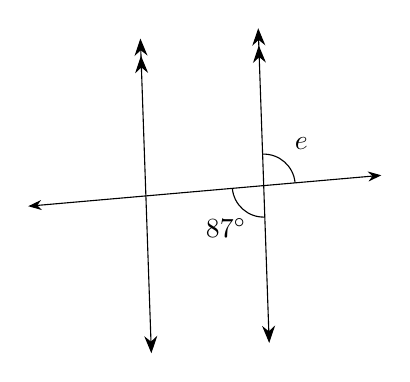
\begin{tikzpicture}[scale=1.0, baseline=(current bounding box.north)]
    \begin{scope}[rotate=5]
      % Draw the first line
      \draw[<->>, >={Stealth[scale=1.3]}, name path=P1] (0, 0) -- (0.20934382497177587, 3.9945181390182953);
      % Draw the second line with the calculated offsets
      \draw[<->>, >={Stealth[scale=1.3]}, name path=P2] (1.5020585189968816, 0) -- (1.7114023439686574, 3.9945181390182953);
      % Draw the transversal through the middle of the parallel lines
      \draw[<->, >=Stealth, name path=P3] (-1.395328087514112, 1.9972590695091477) -- (3.1067304314827697, 1.9972590695091477);
      \path [name intersections={of=P1 and P3,by=A}];
      \path [name intersections={of=P2 and P3,by=B}];
      % Draw the angle
      \coordinate (p1s) at (0, 0);
      \coordinate (p1e) at (0.20934382497177587, 3.9945181390182953);
      \coordinate (p2s) at (1.5020585189968816, 0);
      \coordinate (p2e) at (1.7114023439686574, 3.9945181390182953);
      \coordinate (ts) at (-1.395328087514112, 1.9972590695091477);
      \coordinate (te) at (3.1067304314827697, 1.9972590695091477);
      \draw pic["$e$", draw=black, -, angle eccentricity=1.8, angle radius=0.4cm] {angle=te--B--p2e};
\draw pic["$87^\circ$", draw=black, -, angle eccentricity=1.8, angle radius=0.4cm] {angle=ts--B--p2s};

    \end{scope}
  \end{tikzpicture}
\end{equation}\vspace{1cm}
\begin{equation}
  \text{d} = \text{74}^\circ
  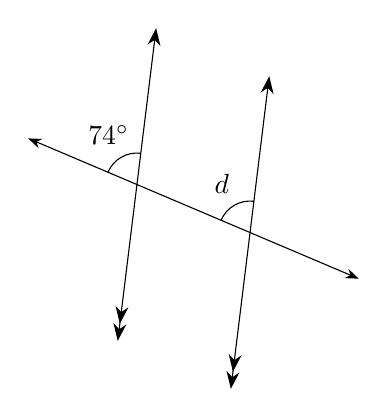
\begin{tikzpicture}[scale=1.0, baseline=(current bounding box.north)]
    \begin{scope}[rotate=157]
      % Draw the first line
      \draw[<->>, >={Stealth[scale=1.3]}, name path=P1] (0, 0) -- (-1.1025494232679962, 3.8450467837532756);
      % Draw the second line with the calculated offsets
      \draw[<->>, >={Stealth[scale=1.3]}, name path=P2] (1.560449153792403, 0) -- (0.4578997305244068, 3.8450467837532756);
      % Draw the transversal through the middle of the parallel lines
      \draw[<->, >=Stealth, name path=P3] (-2.051274711633998, 1.9225233918766378) -- (2.509174442158405, 1.9225233918766378);
      \path [name intersections={of=P1 and P3,by=A}];
      \path [name intersections={of=P2 and P3,by=B}];
      % Draw the angle
      \coordinate (p1s) at (0, 0);
      \coordinate (p1e) at (-1.1025494232679962, 3.8450467837532756);
      \coordinate (p2s) at (1.560449153792403, 0);
      \coordinate (p2e) at (0.4578997305244068, 3.8450467837532756);
      \coordinate (ts) at (-2.051274711633998, 1.9225233918766378);
      \coordinate (te) at (2.509174442158405, 1.9225233918766378);
      \draw pic["$d$", draw=black, -, angle eccentricity=1.8, angle radius=0.4cm] {angle=p1s--A--te};
\draw pic["$74^\circ$", draw=black, -, angle eccentricity=1.8, angle radius=0.4cm] {angle=p2s--B--te};

    \end{scope}
  \end{tikzpicture}
\end{equation}\vspace{1cm}
\begin{equation}
  \text{b} = \text{85}^\circ
  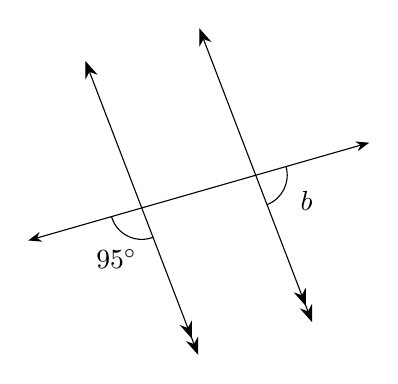
\begin{tikzpicture}[scale=1.0, baseline=(current bounding box.north)]
    \begin{scope}[rotate=196]
      % Draw the first line
      \draw[<->>, >={Stealth[scale=1.3]}, name path=P1] (0, 0) -- (-0.34862297099063294, 3.984778792366982);
      % Draw the second line with the calculated offsets
      \draw[<->>, >={Stealth[scale=1.3]}, name path=P2] (1.5057297563150212, 0) -- (1.1571067853243882, 3.984778792366982);
      % Draw the transversal through the middle of the parallel lines
      \draw[<->, >=Stealth, name path=P3] (-1.6743114854953163, 1.992389396183491) -- (2.8314182708197047, 1.992389396183491);
      \path [name intersections={of=P1 and P3,by=A}];
      \path [name intersections={of=P2 and P3,by=B}];
      % Draw the angle
      \coordinate (p1s) at (0, 0);
      \coordinate (p1e) at (-0.34862297099063294, 3.984778792366982);
      \coordinate (p2s) at (1.5057297563150212, 0);
      \coordinate (p2e) at (1.1571067853243882, 3.984778792366982);
      \coordinate (ts) at (-1.6743114854953163, 1.992389396183491);
      \coordinate (te) at (2.8314182708197047, 1.992389396183491);
      \draw pic["$b$", draw=black, -, angle eccentricity=1.8, angle radius=0.4cm] {angle=p1e--A--ts};
\draw pic["$95^\circ$", draw=black, -, angle eccentricity=1.8, angle radius=0.4cm] {angle=te--B--p2e};

    \end{scope}
  \end{tikzpicture}
\end{equation}\vspace{1cm}
\begin{equation}
  \text{f} = \text{87}^\circ
  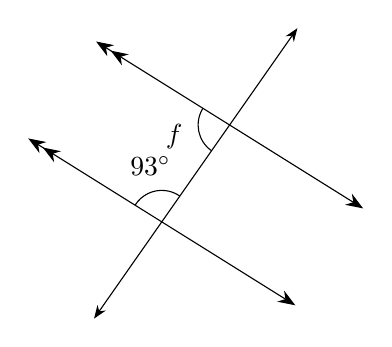
\begin{tikzpicture}[scale=1.0, baseline=(current bounding box.north)]
    \begin{scope}[rotate=55]
      % Draw the first line
      \draw[<->>, >={Stealth[scale=1.3]}, name path=P1] (0, 0) -- (-0.20934382497177537, 3.9945181390182953);
      % Draw the second line with the calculated offsets
      \draw[<->>, >={Stealth[scale=1.3]}, name path=P2] (1.5020585189968816, 0) -- (1.2927146940251062, 3.9945181390182953);
      % Draw the transversal through the middle of the parallel lines
      \draw[<->, >=Stealth, name path=P3] (-1.604671912485888, 1.9972590695091477) -- (2.897386606510994, 1.9972590695091477);
      \path [name intersections={of=P1 and P3,by=A}];
      \path [name intersections={of=P2 and P3,by=B}];
      % Draw the angle
      \coordinate (p1s) at (0, 0);
      \coordinate (p1e) at (-0.20934382497177537, 3.9945181390182953);
      \coordinate (p2s) at (1.5020585189968816, 0);
      \coordinate (p2e) at (1.2927146940251062, 3.9945181390182953);
      \coordinate (ts) at (-1.604671912485888, 1.9972590695091477);
      \coordinate (te) at (2.897386606510994, 1.9972590695091477);
      \draw pic["$f$", draw=black, -, angle eccentricity=1.8, angle radius=0.4cm] {angle=p2e--B--ts};
\draw pic["$93^\circ$", draw=black, -, angle eccentricity=1.8, angle radius=0.4cm] {angle=te--A--p1e};

    \end{scope}
  \end{tikzpicture}
\end{equation}\vspace{1cm}
\begin{equation}
  \text{h} = \text{80}^\circ
  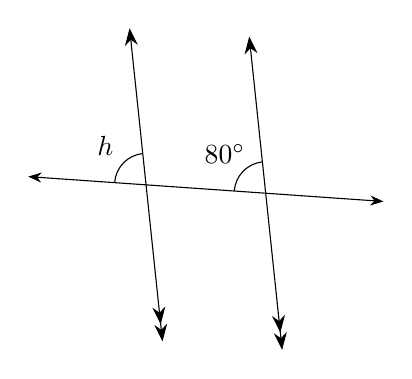
\begin{tikzpicture}[scale=1.0, baseline=(current bounding box.north)]
    \begin{scope}[rotate=176]
      % Draw the first line
      \draw[<->>, >={Stealth[scale=1.3]}, name path=P1] (0, 0) -- (-0.6945927106677212, 3.939231012048832);
      % Draw the second line with the calculated offsets
      \draw[<->>, >={Stealth[scale=1.3]}, name path=P2] (1.5231399178286176, 0) -- (0.8285472071608964, 3.939231012048832);
      % Draw the transversal through the middle of the parallel lines
      \draw[<->, >=Stealth, name path=P3] (-1.8472963553338604, 1.969615506024416) -- (2.675843562494757, 1.969615506024416);
      \path [name intersections={of=P1 and P3,by=A}];
      \path [name intersections={of=P2 and P3,by=B}];
      % Draw the angle
      \coordinate (p1s) at (0, 0);
      \coordinate (p1e) at (-0.6945927106677212, 3.939231012048832);
      \coordinate (p2s) at (1.5231399178286176, 0);
      \coordinate (p2e) at (0.8285472071608964, 3.939231012048832);
      \coordinate (ts) at (-1.8472963553338604, 1.969615506024416);
      \coordinate (te) at (2.675843562494757, 1.969615506024416);
      \draw pic["$h$", draw=black, -, angle eccentricity=1.8, angle radius=0.4cm] {angle=p2s--B--te};
\draw pic["$80^\circ$", draw=black, -, angle eccentricity=1.8, angle radius=0.4cm] {angle=p1s--A--te};

    \end{scope}
  \end{tikzpicture}
\end{equation}\vspace{1cm}
\begin{equation}
  \text{c} = \text{100}^\circ
  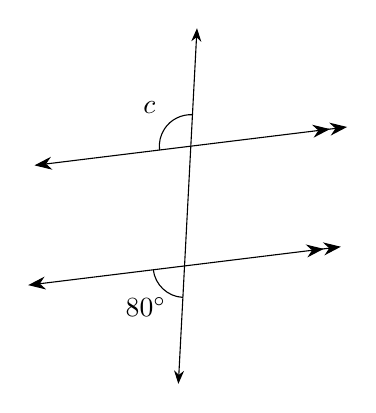
\begin{tikzpicture}[scale=1.0, baseline=(current bounding box.north)]
    \begin{scope}[rotate=267]
      % Draw the first line
      \draw[<->>, >={Stealth[scale=1.3]}, name path=P1] (0, 0) -- (-0.6945927106677212, 3.939231012048832);
      % Draw the second line with the calculated offsets
      \draw[<->>, >={Stealth[scale=1.3]}, name path=P2] (1.5231399178286176, 0) -- (0.8285472071608964, 3.939231012048832);
      % Draw the transversal through the middle of the parallel lines
      \draw[<->, >=Stealth, name path=P3] (-1.8472963553338604, 1.969615506024416) -- (2.675843562494757, 1.969615506024416);
      \path [name intersections={of=P1 and P3,by=A}];
      \path [name intersections={of=P2 and P3,by=B}];
      % Draw the angle
      \coordinate (p1s) at (0, 0);
      \coordinate (p1e) at (-0.6945927106677212, 3.939231012048832);
      \coordinate (p2s) at (1.5231399178286176, 0);
      \coordinate (p2e) at (0.8285472071608964, 3.939231012048832);
      \coordinate (ts) at (-1.8472963553338604, 1.969615506024416);
      \coordinate (te) at (2.675843562494757, 1.969615506024416);
      \draw pic["$c$", draw=black, -, angle eccentricity=1.8, angle radius=0.4cm] {angle=ts--A--p1s};
\draw pic["$80^\circ$", draw=black, -, angle eccentricity=1.8, angle radius=0.4cm] {angle=p2s--B--te};

    \end{scope}
  \end{tikzpicture}
\end{equation}\vspace{1cm}
\begin{equation}
  \text{e} = \text{85}^\circ
  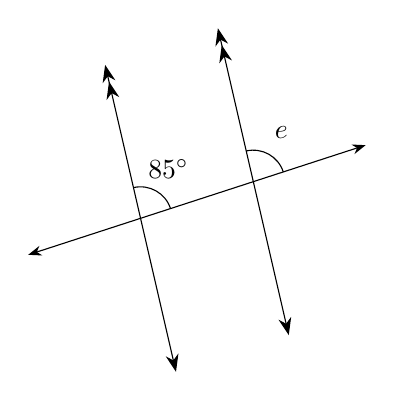
\begin{tikzpicture}[scale=1.0, baseline=(current bounding box.north)]
    \begin{scope}[rotate=18]
      % Draw the first line
      \draw[<->>, >={Stealth[scale=1.3]}, name path=P1] (0, 0) -- (0.34862297099063255, 3.984778792366982);
      % Draw the second line with the calculated offsets
      \draw[<->>, >={Stealth[scale=1.3]}, name path=P2] (1.5057297563150212, 0) -- (1.8543527273056537, 3.984778792366982);
      % Draw the transversal through the middle of the parallel lines
      \draw[<->, >=Stealth, name path=P3] (-1.3256885145046837, 1.992389396183491) -- (3.180041241810337, 1.992389396183491);
      \path [name intersections={of=P1 and P3,by=A}];
      \path [name intersections={of=P2 and P3,by=B}];
      % Draw the angle
      \coordinate (p1s) at (0, 0);
      \coordinate (p1e) at (0.34862297099063255, 3.984778792366982);
      \coordinate (p2s) at (1.5057297563150212, 0);
      \coordinate (p2e) at (1.8543527273056537, 3.984778792366982);
      \coordinate (ts) at (-1.3256885145046837, 1.992389396183491);
      \coordinate (te) at (3.180041241810337, 1.992389396183491);
      \draw pic["$e$", draw=black, -, angle eccentricity=1.8, angle radius=0.4cm] {angle=te--B--p2e};
\draw pic["$85^\circ$", draw=black, -, angle eccentricity=1.8, angle radius=0.4cm] {angle=te--A--p1e};

    \end{scope}
  \end{tikzpicture}
\end{equation}\vspace{1cm}
\begin{equation}
  \text{h} = \text{56}^\circ
  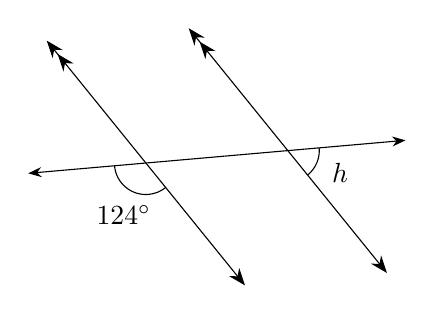
\begin{tikzpicture}[scale=1.0, baseline=(current bounding box.north)]
    \begin{scope}[rotate=5]
      % Draw the first line
      \draw[<->>, >={Stealth[scale=1.3]}, name path=P1] (0, 0) -- (-2.2367716138829867, 3.316150290220167);
      % Draw the second line with the calculated offsets
      \draw[<->>, >={Stealth[scale=1.3]}, name path=P2] (1.809326922755858, 0) -- (-0.4274446911271288, 3.316150290220167);
      % Draw the transversal through the middle of the parallel lines
      \draw[<->, >=Stealth, name path=P3] (-2.618385806941493, 1.6580751451100835) -- (2.190941115814365, 1.6580751451100835);
      \path [name intersections={of=P1 and P3,by=A}];
      \path [name intersections={of=P2 and P3,by=B}];
      % Draw the angle
      \coordinate (p1s) at (0, 0);
      \coordinate (p1e) at (-2.2367716138829867, 3.316150290220167);
      \coordinate (p2s) at (1.809326922755858, 0);
      \coordinate (p2e) at (-0.4274446911271288, 3.316150290220167);
      \coordinate (ts) at (-2.618385806941493, 1.6580751451100835);
      \coordinate (te) at (2.190941115814365, 1.6580751451100835);
      \draw pic["$h$", draw=black, -, angle eccentricity=1.8, angle radius=0.4cm] {angle=p2s--B--te};
\draw pic["$124^\circ$", draw=black, -, angle eccentricity=1.8, angle radius=0.4cm] {angle=ts--A--p1s};

    \end{scope}
  \end{tikzpicture}
\end{equation}\vspace{1cm}
\begin{equation}
  \text{c} = \text{126}^\circ
  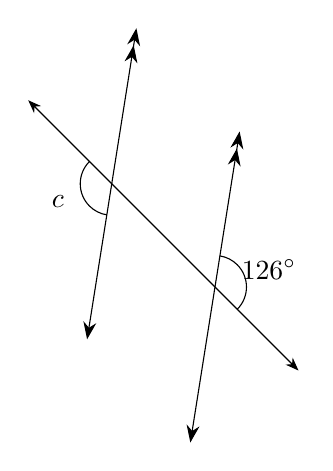
\begin{tikzpicture}[scale=1.0, baseline=(current bounding box.north)]
    \begin{scope}[rotate=315]
      % Draw the first line
      \draw[<->>, >={Stealth[scale=1.3]}, name path=P1] (0, 0) -- (-2.351141009169892, 3.23606797749979);
      % Draw the second line with the calculated offsets
      \draw[<->>, >={Stealth[scale=1.3]}, name path=P2] (1.8541019662496845, 0) -- (-0.4970390429202076, 3.23606797749979);
      % Draw the transversal through the middle of the parallel lines
      \draw[<->, >=Stealth, name path=P3] (-2.6755705045849463, 1.618033988749895) -- (2.1785314616647384, 1.618033988749895);
      \path [name intersections={of=P1 and P3,by=A}];
      \path [name intersections={of=P2 and P3,by=B}];
      % Draw the angle
      \coordinate (p1s) at (0, 0);
      \coordinate (p1e) at (-2.351141009169892, 3.23606797749979);
      \coordinate (p2s) at (1.8541019662496845, 0);
      \coordinate (p2e) at (-0.4970390429202076, 3.23606797749979);
      \coordinate (ts) at (-2.6755705045849463, 1.618033988749895);
      \coordinate (te) at (2.1785314616647384, 1.618033988749895);
      \draw pic["$c$", draw=black, -, angle eccentricity=1.8, angle radius=0.4cm] {angle=ts--A--p1s};
\draw pic["$126^\circ$", draw=black, -, angle eccentricity=1.8, angle radius=0.4cm] {angle=te--B--p2e};

    \end{scope}
  \end{tikzpicture}
\end{equation}\vspace{1cm}

\end{multicols}
\end{document}

